\documentclass[]{ctexbook}
\usepackage{lmodern}
\usepackage{amssymb,amsmath}
\usepackage{ifxetex,ifluatex}
\usepackage{fixltx2e} % provides \textsubscript
\ifnum 0\ifxetex 1\fi\ifluatex 1\fi=0 % if pdftex
  \usepackage[T1]{fontenc}
  \usepackage[utf8]{inputenc}
\else % if luatex or xelatex
  \ifxetex
    \usepackage{xltxtra,xunicode}
  \else
    \usepackage{fontspec}
  \fi
  \defaultfontfeatures{Ligatures=TeX,Scale=MatchLowercase}
\fi
% use upquote if available, for straight quotes in verbatim environments
\IfFileExists{upquote.sty}{\usepackage{upquote}}{}
% use microtype if available
\IfFileExists{microtype.sty}{%
\usepackage{microtype}
\UseMicrotypeSet[protrusion]{basicmath} % disable protrusion for tt fonts
}{}
\usepackage[b5paper,paperwidth=17cm,paperheight=24cm,tmargin=3cm,bmargin=2.4cm,lmargin=3cm,rmargin=2cm]{geometry}
\usepackage[unicode=true]{hyperref}
\hypersetup{
            pdftitle={Steem Engine Handbook},
            pdfauthor={Steem 中文社区集体创作},
            pdfborder={0 0 0},
            breaklinks=true}
\urlstyle{same}  % don't use monospace font for urls
\usepackage{natbib}
\bibliographystyle{apalike}
\usepackage{longtable,booktabs}
% Fix footnotes in tables (requires footnote package)
\IfFileExists{footnote.sty}{\usepackage{footnote}\makesavenoteenv{long table}}{}
\usepackage{graphicx,grffile}
\makeatletter
\def\maxwidth{\ifdim\Gin@nat@width>\linewidth\linewidth\else\Gin@nat@width\fi}
\def\maxheight{\ifdim\Gin@nat@height>\textheight\textheight\else\Gin@nat@height\fi}
\makeatother
% Scale images if necessary, so that they will not overflow the page
% margins by default, and it is still possible to overwrite the defaults
% using explicit options in \includegraphics[width, height, ...]{}
\setkeys{Gin}{width=\maxwidth,height=\maxheight,keepaspectratio}
\IfFileExists{parskip.sty}{%
\usepackage{parskip}
}{% else
\setlength{\parindent}{0pt}
\setlength{\parskip}{6pt plus 2pt minus 1pt}
}
\setlength{\emergencystretch}{3em}  % prevent overfull lines
\providecommand{\tightlist}{%
  \setlength{\itemsep}{0pt}\setlength{\parskip}{0pt}}
\setcounter{secnumdepth}{5}
% Redefines (sub)paragraphs to behave more like sections
\ifx\paragraph\undefined\else
\let\oldparagraph\paragraph
\renewcommand{\paragraph}[1]{\oldparagraph{#1}\mbox{}}
\fi
\ifx\subparagraph\undefined\else
\let\oldsubparagraph\subparagraph
\renewcommand{\subparagraph}[1]{\oldsubparagraph{#1}\mbox{}}
\fi

% set default figure placement to htbp
\makeatletter
\def\fps@figure{htbp}
\makeatother

\usepackage{pdfpages}
\usepackage{wasysym} % insert a smiling and frowning face

\usepackage{booktabs}
\usepackage{longtable}

\usepackage{indentfirst}
\setlength{\parindent}{2em}

\usepackage{framed,color}
\definecolor{shadecolor}{RGB}{248,248,248}

\renewcommand{\textfraction}{0.05}
\renewcommand{\topfraction}{0.8}
\renewcommand{\bottomfraction}{0.8}
\renewcommand{\floatpagefraction}{0.75}

\let\oldhref\href
\renewcommand{\href}[2]{#2\footnote{\url{#1}}}


% \makeatletter
% \newenvironment{kframe}{%
% \medskip{}
% \setlength{\fboxsep}{.8em}
 % \def\at@end@of@kframe{}%
 % \ifinner\ifhmode%
  % \def\at@end@of@kframe{\end{minipage}}%
  % \begin{minipage}{\columnwidth}%
 % \fi\fi%
 % \def\FrameCommand##1{\hskip\@totalleftmargin \hskip-\fboxsep
 % \colorbox{shadecolor}{##1}\hskip-\fboxsep
     % % There is no \\@totalrightmargin, so:
     % \hskip-\linewidth \hskip-\@totalleftmargin \hskip\columnwidth}%
 % \MakeFramed {\advance\hsize-\width
   % \@totalleftmargin\z@ \linewidth\hsize
   % \@setminipage}}%
 % {\par\unskip\endMakeFramed%
 % \at@end@of@kframe}
% \makeatother

% \renewenvironment{Shaded}{\begin{kframe}}{\end{kframe}}

\usepackage{makeidx}
\makeindex

\urlstyle{tt}

\usepackage{amsthm}
\makeatletter
\def\thm@space@setup{%
 \thm@preskip=8pt plus 2pt minus 4pt
 \thm@postskip=\thm@preskip
}
\makeatother


%%%%%%%%%% 生成小贴士目录
% \usepackage{etoolbox}
% \usepackage{amsthm}
% \newtheoremstyle{mystyle}
% {\topsep}{\topsep}{}{}{\bfseries}{:}{\newline}
% {\thmname{#1}\thmnumber{ #2}\thmnote{ (#3)}%
	% \ifstrempty{#3}%
	% {\addcontentsline{def}{subsection}{#1~\themydef}}%
	% {\addcontentsline{def}{subsection}{#1~\themydef~(#3)}}}
% \theoremstyle{mystyle}
% \newtheorem{mydef}{小贴士}
% \makeatletter
% \newcommand\definitionname{小贴士}
% \newcommand\listdefinitionname{小贴士目录}
% \newcommand\listofdefinitions{%
	% \section*{\listdefinitionname}\@starttoc{mydef}}
% \makeatother

\ifxetex
  \usepackage{letltxmacro}
  \setlength{\XeTeXLinkMargin}{1pt}
  \LetLtxMacro\SavedIncludeGraphics\includegraphics
  \def\includegraphics#1#{% #1 catches optional stuff (star/opt. arg.)
    \IncludeGraphicsAux{#1}%
  }%
  \newcommand*{\IncludeGraphicsAux}[2]{%
    \XeTeXLinkBox{%
      \SavedIncludeGraphics#1{#2}%
    }%
  }%
\fi

\newenvironment{rmdblock}[1]
  {\begin{shaded*}
  \begin{itemize}
  \renewcommand{\labelitemi}{
    \raisebox{-.7\height}[0pt][0pt]{
      {\setkeys{Gin}{width=2em,keepaspectratio}\includegraphics{images/icons/#1}}
    }
  }
  \item
  }
  {
  \end{itemize}
  \end{shaded*}
  }
\newenvironment{rmdcaution}
  {\begin{rmdblock}{caution}}
  {\end{rmdblock}}
\newenvironment{rmdinsight}
  {\begin{rmdblock}{insight}}
  {\end{rmdblock}}
\newenvironment{rmdexercise}
  {\begin{rmdblock}{exercise}}
  {\end{rmdblock}}
\newenvironment{rmdexample}
  {\begin{rmdblock}{exeample}}
  {\end{rmdblock}}
\newenvironment{rmdtip}
  {\begin{rmdblock}{tip}}
  {\end{rmdblock}}


%%%%%%% 引用 verbatim 的换行问题
\usepackage{etoolbox}
\usepackage{verbatim}
\makeatletter
\def\@xobeysp{\ }% Or just a space, with a different result
\let\verbatim@nolig@list\empty
\appto\verbatim@font{\raggedright}
\makeatother


\usepackage{xeCJK}% You'd better use the latest version%
%\setCJKmainfont{NSimSun}
\xeCJKsetup{Verb=false}
\normalspacedchars{}
\ExplSyntaxOn
% Hack into xeCJK package if you want to allow linebreaks after (almost) any character.
% Delete this if you don't want that.
\tex_chardef:D \c_fifty = 50 ~
\xeCJK_inter_class_toks:nnn { Default } { Default } { \tex_penalty:D \c_one_hundred }
\xeCJK_inter_class_toks:nnn { Default } { HalfLeft } { \tex_penalty:D \c_fifty }
\xeCJK_inter_class_toks:nnn { Default } { HalfRight } { \tex_penalty:D \c_one_thousand }
\xeCJK_inter_class_toks:nnn { HalfLeft } { Default } { \tex_penalty:D \c_one_thousand }
\xeCJK_inter_class_toks:nnn { HalfLeft } { HalfLeft } { \tex_penalty:D \c_one_thousand }
\xeCJK_inter_class_toks:nnn { HalfLeft } { HalfRight } { \tex_penalty:D \c_one_thousand }
\xeCJK_inter_class_toks:nnn { HalfRight } { Default } { \tex_penalty:D \c_fifty }
\xeCJK_inter_class_toks:nnn { HalfRight } { HalfLeft } { \tex_penalty:D \c_fifty }
\xeCJK_inter_class_toks:nnn { HalfRight } { HalfRight } { \tex_penalty:D \c_one_thousand }
\ExplSyntaxOff
%%%%%%%%%%%%%%%%%%%%%%%%%%%%%%%%%%%%%%%%%%%%%%%%%%%%%%%%%%%%%%%%
% \usepackage{gchords}

% \newcommand\mychords{
% \def\chordsize{1.6mm}   % distance between two frets (and two strings)
% \font\fingerfont=cmr5  % font used for numbering fingers
% \font\namefont=cmr10    % font used for labeling of the chord
% \font\fretposfont=cmr7  % font used for the fret position marker
% \def\dampsymbol{{\tiny$\scriptstyle\times$}} %  `damp this string' marker
% }

% \renewcommand\yoff{3}
% \renewcommand\fingsiz{1.6}

% % upchord
% \newcommand{\AsevenMaj}{\upchord{\chord{t}{x,n,p2,p1,p2,n}{A7+}}}
% \newcommand{\Aseven}{\upchord{\chord{t}{x,n,p2,n,p2,n}{A7}}}
% \newcommand{\A}{\upchord{\chord{t}{x,n,p2,p2,p2,n}{A}}}
% \newcommand{\Am}{\upchord{\chord{t}{n,n,p2,p2,p1,n}{Am}}}
% \newcommand{\Amfive}{\upchord{\chord{{5~}}{p1,p3,p3,p1,p1,p1}{Am(5)}}}
% \newcommand{\Bb}{\upchord{\chord{t}{f1p1,f1p1,p3,p3,p3,f1p1}{$^b$B}}}
% \newcommand{\BmseveN}{\upchord{\chord{t}{x,p2,p4,p3,p3,p2}{Bm7+}}}
% \newcommand{\BmsevenA}{\upchord{\chord{t}{x,n,p4,p4,p3,n}{Bm/A}}}
% \newcommand{\Bmseven}{\upchord{\chord{t}{x,p2,p4,p2,p3,p2}{Bm7}}}
% \newcommand{\Bm}{\upchord{\chord{t}{x,p2,p4,p4,p3,p2}{Bm}}}
% \newcommand{\BM}{\upchord{\chord{t}{f1p2,f1p2,p4,p4,p4,f1p2}{B}}}
% \newcommand{\Bseven}{\upchord{\chord{t}{x,f1p2,p4,f1p2,p4,f1p2,}{B7}}}
% \newcommand{\BMseven}{\upchord{\chord{t}{n,p2,p1,p2,n,p2}{B7}}}
% \newcommand{\BsevenBasDs}{\upchord{\chord{t}{x,x,p1,p2,n,p2}{B7/D\#}}}
% \newcommand{\CM}{\upchord{\chord{t}{n,p3,p2,n,p1,n}{C}}}
% \newcommand{\CssevenLight}{\upchord{\chord{t}{x,p4,p3,p4,p2,x}{C\#7}}}
% \newcommand{\Csthree}{\upchord{\chord{{4~}}{f1p1,f1p1,p3,p3,p3,f1p1}{$^\#$C}}}
% \newcommand{\Cthree}{\upchord{\chord{{3~}}{f1p1,f1p1,p3,p3,p3,f1p1}{C(3)}}}
% \newcommand{\Cseven}{\upchord{\chord{t}{n,p3,p2,p3,p1,n}{C7}}}
% \newcommand{\Cm}{\upchord{\chord{t}{f1p3,f1p3,p5,p5,p4,f1p3}{Cm}}}
% \newcommand{\Csm}{\upchord{\chord{{4~}}{f1p1,f1p1,p3,p3,p2,f1p1}{\#Cm}}}
% \newcommand{\DmBasB}{\upchord{\chord{t}{x,p2,p3,p2,p3,x}{Dm/B}}}
% \newcommand{\DseveN}{\upchord{\chord{t}{x,x,n,p2,p2,p2}{D7+}}}
% \newcommand{\Dseven}{\upchord{\chord{t}{x,x,n,p2,p1,p2}{D7}}}
% \newcommand{\Dsix}{\upchord{\chord{t}{x,x,n,p2,n,p2}{D6}}}
% \newcommand{\D}{\upchord{\chord{t}{x,x,n,p2,p3,p2}{D}}}
% \newcommand{\Dm}{\upchord{\chord{t}{x,x,n,p2,p3,p1}{Dm}}}
% \newcommand{\Eb}{\upchord{\chord{{6~}}{f1p1,f1p1,p3,p3,p3,f1p1}{$^b$E}}}
% \newcommand{\E}{\upchord{\chord{t}{n,p2,p2,p1,n,n}{E}}}
% \newcommand{\Eseven}{\upchord{\chord{{7~}}{f1p1,f1p1,p3,p3,p3,f1p1}{E(7)}}}
% \newcommand{\EseveNNine}{\upchord{\chord{t}{n,f1p2,f1p2,p4,p3,f1p2,}{E79}}}
% \newcommand{\EseveN}{\upchord{\chord{t}{n,p2,p2,p4,p3,p4}{E7}}}
% \newcommand{\EsevenFour}{\upchord{\chord{t}{n,p2,p2,p4,p3,p5}{E7,11}}}
% \newcommand{\Em}{\upchord{\chord{t}{n,p2,p2,n,n,n}{Em}}}
% \newcommand{\F}{\upchord{\chord{t}{f1p1,p3,p3,p2,f1p1,f1p1}{F}}}
% \newcommand{\Fs}{\upchord{\chord{t}{f2p2,p4,p4,p3,f1p2,f1p2}{F\#}}}
% \newcommand{\Fsmin}{\upchord{\chord{t}{f1p2,p4,p4,f1p2,f1p2,f1p2,}{F\#m}}}
% \newcommand{\FsminLight}{\upchord{\chord{t}{x,x,f3p4,f1p2,f1p2,f1p2,}{F\#m}}}
% \newcommand{\FsminBasSeveN}{\upchord{\chord{t}{x,x,f3p3,f1p2,f1p2,f1p2,}{F\#m/E\#}}}
% \newcommand{\FsminBasSeven}{\upchord{\chord{t}{x,x,f2p2,f1p2,f1p2,f1p2,}{F\#m/E}}}
% \newcommand{\FsminSeven}{\upchord{\chord{t}{f1p2,p4,p4,f1p2,p5,f1p2,}{F\#7m}}}
% \newcommand{\GM}{\upchord{\chord{t}{p3,p2,n,n,n,p3}{G}}}
% \newcommand{\Gsminseven}{\upchord{\chord{t}{f2p4,x,f4p4,f4p4,f4p4,f4p4,}{G\#7}}}
% \newcommand{\Gthree}{\upchord{\chord{t}{f1p3,p5,p5,p4,f1p3,f1p3}{G(3)}}}
% \newcommand{\Gm}{\upchord{\chord{{3~}}{f1p1,p3,p3,f1p1,f1p1,f1p1}{Gm}}}
% \newcommand{\Gsm}{\upchord{\chord{{4~}}{f1p1,p3,p3,f1p1,f1p1,f1p1}{\#Gm}}}
% \newcommand{\Gseven}{\upchord{\chord{t}{p3,p2,n,n,n,p1}{G7}}}

% %inline 
% \newcommand{\iAsevenMaj}{\chord{t}{x,n,p2,p1,p2,n}{A7+}}
% \newcommand{\iAseven}{\chord{t}{x,n,p2,n,p2,n}{A7}}
% \newcommand{\iA}{\chord{t}{x,n,p2,p2,p2,n}{A}}
% \newcommand{\iAm}{\chord{t}{n,n,p2,p2,p1,n}{Am}}
% \newcommand{\iAmfive}{\chord{{5~}}{p1,p3,p3,p1,p1,p1}{Am(5)}}
% \newcommand{\iBb}{\chord{t}{f1p1,f1p1,p3,p3,p3,f1p1}{$^b$B}}
% \newcommand{\iBmseveN}{\chord{t}{x,p2,p4,p3,p3,p2}{Bm7+}}
% \newcommand{\iBmsevenA}{\chord{t}{x,n,p4,p4,p3,n}{Bm/A}}
% \newcommand{\iBmseven}{\chord{t}{x,p2,p4,p2,p3,p2}{Bm7}}
% \newcommand{\iBm}{\chord{t}{x,p2,p4,p4,p3,p2}{Bm}}
% \newcommand{\iBM}{\chord{t}{f1p2,f1p2,p4,p4,p4,f1p2}{B}}
% \newcommand{\iBseven}{\chord{t}{x,f1p2,p4,f1p2,p4,f1p2,}{B7}}
% \newcommand{\iBMseven}{\chord{t}{n,p2,p1,p2,n,p2}{B7}}
% \newcommand{\iBsevenBasDs}{\chord{t}{x,x,p1,p2,n,p2}{B7/D\#}}
% \newcommand{\iCM}{\chord{t}{n,p3,p2,n,p1,n}{C}}
% \newcommand{\iCssevenLight}{\chord{t}{x,p4,p3,p4,p2,x}{C\#7}}
% \newcommand{\iCsthree}{\chord{{4~}}{f1p1,f1p1,p3,p3,p3,f1p1}{$^\#$C}}
% \newcommand{\iCthree}{\chord{{3~}}{f1p1,f1p1,p3,p3,p3,f1p1}{C(3)}}
% \newcommand{\iCseven}{\chord{t}{n,p3,p2,p3,p1,n}{C7}}
% \newcommand{\iCm}{\chord{t}{f1p3,f1p3,p5,p5,p4,f1p3}{Cm}}
% \newcommand{\iCsm}{\chord{{4~}}{f1p1,f1p1,p3,p3,p2,f1p1}{\#Cm}}
% \newcommand{\iDmBasB}{\chord{t}{x,p2,p3,p2,p3,x}{Dm/B}}
% \newcommand{\iDseveN}{\chord{t}{x,x,n,p2,p2,p2}{D7+}}
% \newcommand{\iDseven}{\chord{t}{x,x,n,p2,p1,p2}{D7}}
% \newcommand{\iDsix}{\chord{t}{x,x,n,p2,n,p2}{D6}}
% \newcommand{\iD}{\chord{t}{x,x,n,p2,p3,p2}{D}}
% \newcommand{\iDm}{\chord{t}{x,x,n,p2,p3,p1}{Dm}}
% \newcommand{\iEb}{\chord{{6~}}{f1p1,f1p1,p3,p3,p3,f1p1}{$^b$E}}
% \newcommand{\iE}{\chord{t}{n,p2,p2,p1,n,n}{E}}
% \newcommand{\iEseven}{\chord{{7~}}{f1p1,f1p1,p3,p3,p3,f1p1}{E(7)}}
% \newcommand{\iEseveNNine}{\chord{t}{n,f1p2,f1p2,p4,p3,f1p2,}{E79}}
% \newcommand{\iEseveN}{\chord{t}{n,p2,p2,p4,p3,p4}{E7}}
% \newcommand{\iEsevenFour}{\chord{t}{n,p2,p2,p4,p3,p5}{E7,11}}
% \newcommand{\iEm}{\chord{t}{n,p2,p2,n,n,n}{Em}}
% \newcommand{\iF}{\chord{t}{f1p1,p3,p3,p2,f1p1,f1p1}{F}}
% \newcommand{\iFs}{\chord{t}{f2p2,p4,p4,p3,f1p2,f1p2}{F\#}}
% \newcommand{\iFsmin}{\chord{t}{f1p2,p4,p4,f1p2,f1p2,f1p2,}{F\#m}}
% \newcommand{\iFsminLight}{\chord{t}{x,x,f3p4,f1p2,f1p2,f1p2,}{F\#m}}
% \newcommand{\iFsminBasSeveN}{\chord{t}{x,x,f3p3,f1p2,f1p2,f1p2,}{F\#m/E\#}}
% \newcommand{\iFsminBasSeven}{\chord{t}{x,x,f2p2,f1p2,f1p2,f1p2,}{F\#m/E}}
% \newcommand{\iFsminSeven}{\chord{t}{f1p2,p4,p4,f1p2,p5,f1p2,}{F\#7m}}
% \newcommand{\iGM}{\chord{t}{p3,p2,n,n,n,p3}{G}}
% \newcommand{\iGsminseven}{\chord{t}{f2p4,x,f4p4,f4p4,f4p4,f4p4,}{G\#7}}
% \newcommand{\iGthree}{\chord{t}{f1p3,p5,p5,p4,f1p3,f1p3}{G(3)}}
% \newcommand{\iGm}{\chord{{3~}}{f1p1,p3,p3,f1p1,f1p1,f1p1}{Gm}}
% \newcommand{\iGsm}{\chord{{4~}}{f1p1,p3,p3,f1p1,f1p1,f1p1}{\#Gm}}
%\usepackage{CJK,CJKnumb,CJKulem}  
%\newcommand{\kai}{\CJKfamily{kai}}       % 楷体
\usepackage{fancyhdr}
% Clear the header and footer
\fancyhead{}
\fancyfoot{}
\fancypagestyle{plain}{% 每章首页无页码
	\fancyhf{}
	\renewcommand{\headrulewidth}{0pt}
	\renewcommand{\footrulewidth}{0pt}
}
%\fancyhead[LE]{\small \kaishu \leftmark}
\fancyhead[LE]{\small \kaishu Steem 指南}
\fancyhead[RO]{\small \kaishu \leftmark}
\fancyfoot[LE, RO]{\thepage}
%\fancyfoot[RE]{\small \kaishu 学 R}
%\fancyfoot[LO]{\small \kaishu 零基础学习 R 语言}
%\renewcommand{\footrulewidth}{0.4pt} % 页脚横线
\pagestyle{fancy}

\frontmatter

\title{Steem Engine Handbook}
\author{Steem 中文社区集体创作}
\date{2019-07-18}

\begin{document}
%\maketitle

\begin{titlepage}
%    
\includegraphics[width=17cm]{images/cover.jpg}

\includepdf{images/cover.jpg}
\end{titlepage}

\setlength{\abovedisplayskip}{-5pt}
\setlength{\abovedisplayshortskip}{-5pt}

{
\setcounter{tocdepth}{1}
\tableofcontents
}

% \tableofcontents
% \clearpage
% \listofdefinitions

\hypertarget{index}{%
\chapter*{前言}\label{index}}
\addcontentsline{toc}{chapter}{前言}

自盘古开天地以来\ldots{}\ldots{}

\begin{quote}
(未完待续)
\end{quote}

\mainmatter

\hypertarget{start}{%
\chapter{入门 Getting Started}\label{start}}

\hypertarget{se-basics}{%
\section{Steem Engine 入门}\label{se-basics}}

\hypertarget{-steem-engine}{%
\subsection{什么是 Steem Engine?}\label{-steem-engine}}

首先,你或许可以参考 \href{https://steem-engine.com/?p=faq}{Steem Engine的FAQ} 了解它对自己的介绍 \ldots{}..

\begin{center}\rule{0.5\linewidth}{\linethickness}\end{center}

\hypertarget{se-operation}{%
\section{Steem Engine 常用操作}\label{se-operation}}

\hypertarget{purchase-token}{%
\subsection[怎样在 Steem Engine 购买代币? ]{\texorpdfstring{怎样在 Steem Engine 购买代币? \footnote{作者:@ericet,原文链接:\url{https://busy.org/@ericet/steem-engine-7mkxyo7yjn}}}{怎样在 Steem Engine 购买代币? }}\label{purchase-token}}

众所周知,Steemit Inc的SMT计划一拖再拖。终于,大家受不了这么漫长的等待,\href{mailto:由@aggroed带头开始社区自己搞SMT}{\nolinkurl{由@aggroed带头开始社区自己搞SMT}}。

几个月时间,steem-engine就上线了\textasciitilde{} 上线后有很多DApps,社区在上面创建了属于自己的币。

\href{mailto:比如@tipu的TPU}{\nolinkurl{比如@tipu的TPU}},韩国社区的JJM,YES,STEEMSC 等币已经在steem-engine上面拥有很多交易量了

如果你也对steem-engine上面的币心动,想着购买,这里介绍一下大概的购买流程。

登录 steem-engine.com

有2种登录方式:
* 安装Chrome/Brave/Firefox浏览器插件steem keychain。
推荐keychain。很方便的插件。相当于集很多功能的STEEM钱包。具体怎么安装设置keychain,可以看看这篇帖子:\url{https://busy.org/@ericet/steempeak-w0yo19h857}
* posting key登录
直接输入steem id和发帖密钥登录

充值

登录后,点击页面上方的``Market'',然后``Deposit''(充值)

之前只支持STEEM充值,没想到1个月不到已经可以支持LTC,BTC,BCH,DOGE了
选择你拥有的币的种类,按照提示充值。
需要注意的是,提现充值需要收取1\%的手续费。但是交易是没有费用的

等你充值成功后,在你的钱包里会多了一个STEEMP的币。
这个币是1:1 和STEEM挂钩的,任何时候充值提现,1STEEMP都等于1STEEM。

交易

充好值后,点击页面上方的``TOKENS'',查看所有的币。
选择你想购买的币,点击图上双箭头的标志。

进入交易页面。可以选择买入币(Buy XXX)或者卖出币(Sell XXX)。价格是按STEEM算的

填入自己心仪的价格后,就可以点击``Buy''或者``Sell''按钮

好了,单子挂好了,就等交易成功了。

虽然目前steem-engine上有很多乱七八糟的币,但是引入币的概念对DApp还是社区的发展都是有益的。

\hypertarget{wallet}{%
\subsection[钱包常用操作 ]{\texorpdfstring{钱包常用操作 \footnote{作者:@shine.wong,原文链接:\url{https://busy.org/@shine.wong/steem-engine}}}{钱包常用操作 }}\label{wallet}}

锁仓 Stake

登录\href{https://steem-engine.com}{steem-engine}进入你的钱包(Wallet)。

主要界面是英文大家用起来不熟悉而已,其实鼠标悬停,最右边的几个图标都有英文简介(貌似可以有7个图标这里就5个)。

\begin{figure}
\centering

\includegraphics{images/chapter_01_0/SJmJHVre-image.png}
\caption{image.png}
\end{figure}

如图最右边你看到一个锁着的按钮,表示你有未锁仓的ttoken可以操作锁仓。锁仓几乎就是power down

当你按下之后,更具提示输入你要锁仓的金额就可以了!
确认锁仓后你会看到
\includegraphics{images/chapter_01_0/IpSBaCeP-image.png}解锁的图标,当你需要解除锁仓时,可以点击这个图标,类似power up。

需要注意的是每种token的解锁时效是不一样的,锁仓前最好了了解一下哟!

\hypertarget{scot-basics}{%
\section{SCOT 入门}\label{scot-basics}}

\hypertarget{purchase-token}{%
\subsection[什么是 SCOT? ]{\texorpdfstring{什么是 SCOT? \footnote{作者:@ericet,原文链接:\url{https://busy.org/@ericet/steem-engine-7mkxyo7yjn}}}{什么是 SCOT? }}\label{purchase-token}}

\href{mailto:社区的行动派大佬@aggroed继steemmonsters}{\nolinkurl{社区的行动派大佬@aggroed继steemmonsters}},steem-engine, STO后又出新作\textasciitilde{} SCOT( Smart Contract Organizational Token) SCOT Testing underway!!! Are you ready for your own token that can distribute like Steem?

这个SCOT是什么呢?其实就是steemit inc从几年前一直鼓吹的SMT。

SMT的概念是,每个社区可以在STEEM区块链上创建属于自己的币。每个社区可以创建属于自己的steemit.com前端,文章的收益除了STEEM外还有自己创建的币。

打个比方,steempress发了SMT。所有通过steempress插件发布的文章除了STEEM收益外,还可以获得steempress自己的代币。steempress的代币可以通过steem-engine交易成其他货币(BTC,LTC,STEEM等)。获得的steempress代币的多少,取决于给你点赞人持有的steempress的代币多少。

SCOT就是拿了SMT的理念,把他变成现实。

但是和SMT不一样的是,SCOT是建立在STEEM的第二层,而不是像SMT那样全部建立在STEEM链上。这样做的好处是:

\begin{itemize}
\tightlist
\item
  不需要硬分叉。如果建立在STEEM链上需要硬分叉,大家也知道上回的硬分叉给STEEM带来多少问题吧。
\item
  快捷。修改STEEM代码是非常花费时间。
\end{itemize}

SCOT会带给STEEM什么好处呢?

\begin{itemize}
\tightlist
\item
  不需要分叉来建立新的代币。很多steem的分叉,比如weku,whaleshares,bearshares,golos都是steem的分叉,都有属于自己的代币。如果STEEM拥有SMT的属性,那这些平台就只要基于STEEM创建一个自己的代币和平台,而不需要来个分叉创建平台和代币。
\item
  每个社区将可以按照自己的规则管理自己的社区。
\end{itemize}

很高兴有机会当SCOT的测试员,抢先体验了一下SCOT。

aggroed发了72000 SCOT用于测试,要求随便发帖加上scottest的标签,并且给scottest标签底下的帖子点赞

测试版的steem-engine多了Stake和unstake的选项。按照我自己的理解,stack就等于power up,unstack等于power down

帖子获得的SCOT的多少取决于给你点赞的人拥有多少stake的SCOT(相当于拥有多少SP)

unstake需要多久才能提现这个应该是可以设置的,还有帖子SCOT收益部分多久结算也应该是可以设置的。可能帖子收益和审查收益的比例也可以设置(?) 很多种未知的可能。

看了上面的设置,CN区完全可以出一个属于自己的SCOT,各种规则由CN区自己做主。比如steemcleaners按照他们的标准踩CN区的帖子,这里完全可以CN区自己管理。毕竟每个社区的标准不同。

\hypertarget{scotbot-settings}{%
\subsection[ScotBot 的设定 ]{\texorpdfstring{ScotBot 的设定 \footnote{作者:@ericet,原文链接:\url{https://busy.org/@ericet/scotbot-1b94mfpktn/}}}{ScotBot 的设定 }}\label{scotbot-settings}}

\href{mailto:今天@aggroed介绍了ScotBot的具体设置}{\nolinkurl{今天@aggroed介绍了ScotBot的具体设置}}:Scot and Scotbot Part III: Scotbot settings.

主要有以下这些设置:

\begin{itemize}
\tightlist
\item
  author\_curve\_exponent:作者收益可选线性(1)或者曲线(2)
\item
  author\_reward\_percentage: 作者获得帖子收益的百分百(0-100). 比如现在steem的设置是75\%给帖子作者,25\%给curators。
\item
  cashout\_window\_days: 帖子结算天数(0.1 - 365)。steem目前的设置是7天,如果这个参数改成1的话,就是每天帖子1结算。
\item
  curation\_curve\_exponent: Curator收益可选普通线性(0.5) - 极端线性(2.0)
\item
  downvote\_power\_consumption: 踩后帖子扣除收益的百分百(1 - 10000 ) 100代表1\%,10000代表100\%。如果要设置成和steem现在的设置一样,踩和点赞耗费同样多的VP,downvote\_power\_consumption 和 vote\_power\_consumption 要设置成一样的参数。
\item
  downvote\_regeneration\_seconds: 踩的奖金池恢复速度。如果要和steem的一样,设置参数为432000(6天)。如果不想要这个设定,设置成-1.
\item
  issue\_token: 是否发行代币。选择true或者false
\item
  json\_metadata\_key: 这个选项目前只能填``tags'',意思是,在特定的标签里的帖子才会获得代币。未来会添加``urls''这个选项,意思是在这个链接底下的帖子将会获得代币。
\item
  json\_metadata\_value: 因为目前只有``tags''的选项,所有这里输入你要设置哪个标签底下的帖子才会获得代币。比如设置``cn'',发cn标签的帖子将会自动获得代币。
\item
  reduction\_every\_n\_block: 多少个区块减少比例。可以设置10512000(一年)。一年后,将减少派送的代币的比例。
\item
  reduction\_percentage: 减少的比例。 Steem现在的设置是0.5\%,意思是每年生出的STEEM数量减少大概0.5\%。
\item
  rewards\_token: 每生产X个区块,有多少代币放入奖金池。Steem目前的设定好像是每3个区块将产生1个STEEM
\item
  rewards\_token\_every\_n\_block": 设置X区块。比如设置成10,就是每10个区块将生产X个代币。
\item
  token: 代币的符号
\item
  token\_account: 代币账号
\item
  vote\_power\_consumption: 点赞的消耗率。Steem现在是2,意思是每次满赞耗费2\%
\item
  vote\_regeneration\_seconds": 需要多久时间恢复VP。STEEM的设置是432000(5天),就是每天恢复20\%,5天恢复。
\end{itemize}

从以上的设置来看,SCOT给了社区/DApps很多的权利来选择自己想要的参数。

\hypertarget{theory}{%
\chapter{原理 Theory}\label{theory}}

\begin{enumerate}
\def\labelenumi{\arabic{enumi}.}
\tightlist
\item
  什么是 Steem Smart Contracts?
\item
  什么是 SCOT (Smart Contract Organizational Token)?
\item
  什么是 Nitrous?
\end{enumerate}

\begin{quote}
(未完待续)
\end{quote}

\hypertarget{tribes}{%
\chapter{社群 Tribes}\label{tribes}}

\hypertarget{whats-tribes}{%
\section{什么是 SCOT 社群 (SCOT Tribes)?}\label{whats-tribes}}

\hypertarget{tribes-config}{%
\section{SCOT 社群设定总览}\label{tribes-config}}

本节介绍 SCOT 社区的核心设定,帮助 SCOT 社区的成员们快速了解和比较各个社区和相应货币的关键设定。

\begin{longtable}[]{@{}llllllllll@{}}
\toprule
社区 & Token & 网站 & 标签 & 结算时间(天) & 点赞时间(天) & 取消锁仓时间(天) & 取消代理时间(天) & 作者收益曲线 & 点赞收益曲线\tabularnewline
\midrule
\endhead
Steemcoinpan & SCT & \url{https://www.steemcoinpan.com} & sct & 3 & 2 & 3 & 3 & 1.3 & 0.9\tabularnewline
\bottomrule
\end{longtable}

\hypertarget{intro-to-tribes}{%
\section{SCOT 社群(Tribes)介绍}\label{intro-to-tribes}}

\hypertarget{sct}{%
\subsection{SCT}\label{sct}}

\hypertarget{aaa}{%
\subsection{AAA}\label{aaa}}

\hypertarget{token}{%
\chapter{货币 Token}\label{token}}

本章节涉及的常用问题有:

\begin{enumerate}
\def\labelenumi{\arabic{enumi}.}
\tightlist
\item
  Steem Engine 上的 Token 从何而来?
\item
  什么是 ENG?它是如何被使用的?
\item
  什么是JJM(Jiangjiangman)?它为什么火了?
\item
  什么是红包币?EMFOUR4 / EM
\item
  NBC 新手币 牛掰在哪里?
\end{enumerate}

\hypertarget{nbc-}{%
\section[NBC 新手币 ]{\texorpdfstring{NBC 新手币 \footnote{作者:@ericet;编辑:@minloulou;原文链接:\url{https://steempeak.com/cn/@ericet/steem-enginenbc-8gramkt1en}}}{NBC 新手币 }}\label{nbc-}}

NBC是什麼

NBC是\href{https://steempeak.com/@team-cn}{@team-cn}在steem-engine上发的一款代币。目的是取代对SBI(Steem Basic Income)的依赖,奖励社区积极分子,好文作者和在背后努力的各种编辑(好声音,steem手册,寻宝团,飞鸽传书等)

目前市场价格1 NBC = 1 STEEM,在市面上流通的NBC数量大概5000。

持有NBC的好处

\begin{itemize}
\item
  每日点赞,持有新手币者,将会获得\href{https://steempeak.com/@team-cn}{@team-cn}每日一帖的点赞; 目前\href{https://steempeak.com/@team-cn}{@team-cn}账号大概有20000SP, 持有2 NBC每日会获得2\% team-cn点赞(相当于400sp),如果把`cn' 作为首标签,还可以额外获得2\%点赞(相当于800sp)。
\item
  收益分红,每日按锁仓币的比重,分享 \href{https://steempeak.com/@team-cn}{@team-cn}的SBD/STEEM收益分红; \href{https://steempeak.com/@team-cn}{@team-cn}的收益主要来自飞鸽传书50\%收益,寻宝团50\%收益,小卖部30\%收益,\href{https://steempeak.com/@teamcn-fund}{@teamcn-fund}每日发帖收益,还有少量来自\href{https://steempeak.com/@team-cn}{@team-cn}发帖收益。 由于收益时高时低,并不能准确估计年回报率是多少。但是超过30\%年利率是肯定的。 以NBC的长期支持者嘉楠哥\href{https://steempeak.com/@jianan}{@jianan}的NBC持有算一下年回报率:
\end{itemize}

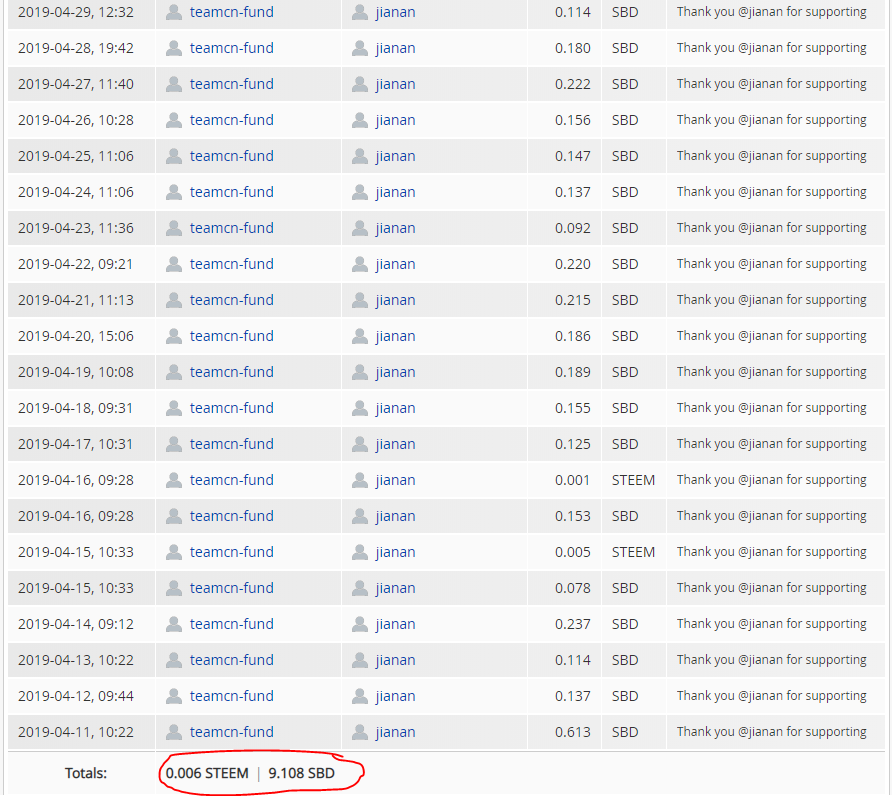
\includegraphics{images/chapter_04_0/ZOiFJBz.png}

嘉楠哥持有300 NBC 2个月,总共获得0.006 STEEM和9.108 SBD,按照目前1 SBD = 2.5 STEEM计算,2个月获得22.776 STEEM分红。一年的年利率差不多45.55\%。还没算上发帖获得的点赞。

目前从原持有NBC就可以获得STEEM/SBD分红改成了只有锁仓NBC才会有分红后,锁仓NBC的用户的年利率将大大提高。

比如今天嘉楠哥获得0.33 SBD,换算成steem 是0.825 steem。一年回报率达到了100\%!(需要更多数据支持,但是超过50\%年回报率是妥妥的!)

\begin{itemize}
\tightlist
\item
  容易变现,不需如SP般等待13周的power down周期; 很多项目需要把steem power up后才能通过代理获得每日点赞/分红。如果你想提现走人,需要5日把SP抽回,并且13周时间全部power down。这提现的周期实在有点太长了。 但是如果你持有NBC,你同样可以获得每日点赞/分红。如果你想提现走人,把手上的NBC通过steem-engine出售换成steem就可以提款走人了。
\item
  容易转换币权,可透过交易平台 Steem-Engine.com转赠他人。 一般如果你想把SP当成礼物送给他人,需要代理SP给他。这代理不是永久的,如果对方把SP收回,你的SP就没了。 如果持有NBC,你可以把NBC作为一个奖励或者礼物永久的送给他人。
\item
  持有NBC获得\href{https://steempeak.com/@sct.teamcn}{@sct.teamcn}点赞
\end{itemize}

\href{https://steempeak.com/@sct.teamcn}{@sct.teamcn}这个账号目前有928 staked SCT. 专门用于给持有NBC的用户的sct帖子点赞。会不断增加锁仓SCT的数量来提高点赞。算是给NBC持有者的额外福利。

NBC的价值在哪里?

NBC的价值来自\href{https://steempeak.com/@team-cn}{@team-cn}. 只要\href{https://steempeak.com/@team-cn}{@team-cn}继续下去,NBC就会有价值。

目前支撑NBC的价值的是来自各种\href{https://steempeak.com/@team-cn}{@team-cn}的基础设施,比如\href{https://steempeak.com/@cn-curation}{@cn-curation},\href{https://steempeak.com/@cn-activity}{@cn-activity},\href{https://steempeak.com/@teamcn-shop}{@teamcn-shop},\href{https://steempeak.com/@teamcn-fund}{@teamcn-fund}。

\href{https://steempeak.com/@team-cn}{@team-cn} 也没有跑路的风险,因为这是个公益项目,没有盈利也没有亏损。获得的收益也全部回报给社区和持有NBC者。

怎么获得NBC?

\begin{itemize}
\tightlist
\item
  通过steem-engine市场购买 目前有少量的NBC可以在市场上购买,最低卖价是1.04 STEEM。 购买链接:\url{https://steem-engine.com/?p=market\&t=NBC}
\end{itemize}

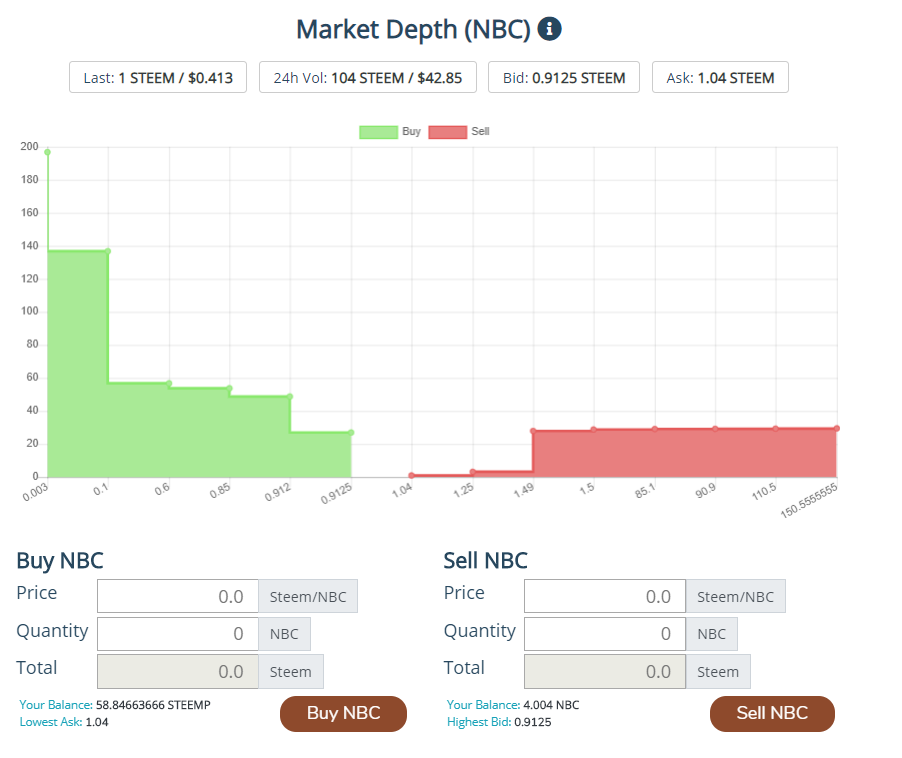
\includegraphics{images/chapter_04_0/rS3MtvD.png}

\begin{itemize}
\tightlist
\item
  通过代理SP给\href{https://steempeak.com/@team-cn}{@team-cn}获得 代理SP给team-cn除了可以获得每日点赞外,还可以获得每日0.05\%的NBC利息(一年20\%复利)
  使用下面链接代理给\href{https://steempeak.com/@team-cn}{@team-cn}: \href{https://steemconnect.com/sign/delegateVestingShares?delegatee=team-cn\&vesting_shares=10\%20SP}{10SP}, \href{https://steemconnect.com/sign/delegateVestingShares?delegatee=team-cn\&vesting_shares=20\%20SP}{20SP}, \href{https://steemconnect.com/sign/delegateVestingShares?delegatee=team-cn\&vesting_shares=50\%20SP}{50SP}, \href{https://steemconnect.com/sign/delegateVestingShares?delegatee=team-cn\&vesting_shares=100\%20SP}{100SP}, \href{https://steemconnect.com/sign/delegateVestingShares?delegatee=team-cn\&vesting_shares=200\%20SP}{200SP}, \href{https://steemconnect.com/sign/delegateVestingShares?delegatee=team-cn\&vesting_shares=300\%20SP}{300SP}, \href{https://steemconnect.com/sign/delegateVestingShares?delegatee=team-cn\&vesting_shares=400\%20SP}{400SP}, \href{https://steemconnect.com/sign/delegateVestingShares?delegatee=team-cn\&vesting_shares=500\%20SP}{500SP}, \href{https://steemconnect.com/sign/delegateVestingShares?delegatee=team-cn\&vesting_shares=1000\%20SP}{1,000SP}, \href{https://steemconnect.com/sign/delegateVestingShares?delegatee=team-cn\&vesting_shares=5000\%20SP}{5,000SP}, \href{https://steembottracker.com/delegation.html?delegatee=team-cn}{其他数量}
\item
  通过参与社区建设,活动,写好文获得
\end{itemize}

\begin{enumerate}
\def\labelenumi{\arabic{enumi}.}
\tightlist
\item
  参与不同社区活动活动,比如完成5期\href{https://steempeak.com/@team-cn}{@team-cn}每周一发布的作业就可以获得1 NBC。参与好声音,参与steem手册编辑都可以获得NBC奖励。
\item
  飞鸽传书每天会选2篇好文给予点赞并且每个作者获得1 NBC
\item
  担任好声音,寻宝团,steem手册,飞鸽传书的编辑获得NBC
\end{enumerate}

NBC是社区的良心项目,设计的本意是让\href{https://steempeak.com/@team-cn}{@team-cn}可以有更多的SP支持一些社区项目,并且让好文作者,参与社区建设的人获得一些回报。大家可以放心购买并持有。

想了解更多,可以看:
- \href{https://steempeak.com/cn/@team-cn/newbies-coin-nbc-white-paper-version-1-0-nbc-1-0}{NBC的白皮书}
- \href{https://steempeak.com/@team-cn/nbc-201964nbcthetermschangeofnbcdailydividends-82gxnr3ys4}{【新手币 NBC公告 - 2019年6月4日】有关新手币 NBC 分红条款变更/The Terms Change of NBC Daily Dividends ---}

\hypertarget{shop}{%
\section{SHOP币}\label{shop}}

\begin{enumerate}
\def\labelenumi{\arabic{enumi}.}
\tightlist
\item
  SHOP币 有几种玩法?
\end{enumerate}

\begin{quote}
(未完待续)
\end{quote}

\hypertarget{tool}{%
\chapter{工具 Tool}\label{tool}}

\begin{longtable}[]{@{}lll@{}}
\toprule
\begin{minipage}[b]{0.30\columnwidth}\raggedright
名称\strut
\end{minipage} & \begin{minipage}[b]{0.30\columnwidth}\raggedright
链接\strut
\end{minipage} & \begin{minipage}[b]{0.30\columnwidth}\raggedright
说明\strut
\end{minipage}\tabularnewline
\midrule
\endhead
\begin{minipage}[t]{0.30\columnwidth}\raggedright
Steem Engine CN版\strut
\end{minipage} & \begin{minipage}[t]{0.30\columnwidth}\raggedright
\url{https://steem-engine.netlify.com}\strut
\end{minipage} & \begin{minipage}[t]{0.30\columnwidth}\raggedright
CN区专用\strut
\end{minipage}\tabularnewline
\begin{minipage}[t]{0.30\columnwidth}\raggedright
Block Explorer\strut
\end{minipage} & \begin{minipage}[t]{0.30\columnwidth}\raggedright
\url{https://steem-engine.rocks}\strut
\end{minipage} & \begin{minipage}[t]{0.30\columnwidth}\raggedright
steem-engine的steemd\strut
\end{minipage}\tabularnewline
\begin{minipage}[t]{0.30\columnwidth}\raggedright
Token的动态\strut
\end{minipage} & \begin{minipage}[t]{0.30\columnwidth}\raggedright
\url{https://steem-engine.rocks/transactions?symbol=\%7Btoken\%7D}\strut
\end{minipage} & \begin{minipage}[t]{0.30\columnwidth}\raggedright
举例:\url{https://steem-engine.rocks/transactions?symbol=SCT}\strut
\end{minipage}\tabularnewline
\begin{minipage}[t]{0.30\columnwidth}\raggedright
账户的动态\strut
\end{minipage} & \begin{minipage}[t]{0.30\columnwidth}\raggedright
\url{https://steem-engine.rocks/@\%7Bid\%7D}\strut
\end{minipage} & \begin{minipage}[t]{0.30\columnwidth}\raggedright
举例:\href{https://steem-engine.rocks/@aggroed}{https://steem-engine.rocks/\citet{aggroed}}\strut
\end{minipage}\tabularnewline
\begin{minipage}[t]{0.30\columnwidth}\raggedright
Token的持有和锁仓\strut
\end{minipage} & \begin{minipage}[t]{0.30\columnwidth}\raggedright
\url{https://steem-engine.rocks/tokens/\%7Btoken\%7D/richlist}\strut
\end{minipage} & \begin{minipage}[t]{0.30\columnwidth}\raggedright
举例:\url{https://steem-engine.rocks/tokens/SCT/richlist}\strut
\end{minipage}\tabularnewline
\begin{minipage}[t]{0.30\columnwidth}\raggedright
交易订单\strut
\end{minipage} & \begin{minipage}[t]{0.30\columnwidth}\raggedright
\url{https://steem-engine.rocks/open_orders/@\%7Bid\%7D}\strut
\end{minipage} & \begin{minipage}[t]{0.30\columnwidth}\raggedright
举例:\href{https://steem-engine.rocks/open_orders/@aggroed}{https://steem-engine.rocks/open\_orders/\citet{aggroed}}\strut
\end{minipage}\tabularnewline
\begin{minipage}[t]{0.30\columnwidth}\raggedright
Wallet\strut
\end{minipage} & \begin{minipage}[t]{0.30\columnwidth}\raggedright
\url{https://steem-engine.com/?p=balances}\strut
\end{minipage} & \begin{minipage}[t]{0.30\columnwidth}\raggedright
举例:\url{https://steem-engine.com/?p=balances\&a=robertyan}\strut
\end{minipage}\tabularnewline
\begin{minipage}[t]{0.30\columnwidth}\raggedright
Market\strut
\end{minipage} & \begin{minipage}[t]{0.30\columnwidth}\raggedright
\url{https://steem-engine.com/?p=market\&t=\%7Btoken\%7D}\strut
\end{minipage} & \begin{minipage}[t]{0.30\columnwidth}\raggedright
举例: \url{https://steem-engine.com/?p=market\&t=SCT}\strut
\end{minipage}\tabularnewline
\begin{minipage}[t]{0.30\columnwidth}\raggedright
VP\strut
\end{minipage} & \begin{minipage}[t]{0.30\columnwidth}\raggedright
\url{https://economicstudio.github.io/vp/a=\%7Busername\%7D\&t=\%7Btoken\%7D}\strut
\end{minipage} & \begin{minipage}[t]{0.30\columnwidth}\raggedright
举例: \url{https://economicstudio.github.io/vp/?a=robertyan\&t=SCT}\strut
\end{minipage}\tabularnewline
\bottomrule
\end{longtable}

\begin{quote}
(未完待续)
\end{quote}

\hypertarget{developer}{%
\chapter{开发 Developers}\label{developer}}

\hypertarget{business}{%
\section{创建服务或社群}\label{business}}

\hypertarget{create-scot-tribes}{%
\subsection[如何创建 SCOT 社群 ]{\texorpdfstring{如何创建 SCOT 社群 \footnote{作者:@ericet; 编辑:@robertyan; 原文链接: \url{https://busy.org/@ericet/scot-nayl5hcpvy}}}{如何创建 SCOT 社群 }}\label{create-scot-tribes}}


\includegraphics{images/chapter_06_0/Ta8eNake-image.png}
(Source: \href{https://pixabay.com/vectors/social-media-connections-networking-3846597/}{Pixabay})

越来越多的团体或者个人开始创建自己的SCOT社群了。大家在创建自己的社群之前,问问自己下面几个问题,看看是否自己已经准备好了

创建一个SCOT社群并不便宜,所以需要有足够的资金起步。

最基础的配置(2100 ENG):

\begin{itemize}
\tightlist
\item
  创建代币:100 ENG
\item
  购买ScotBot:1000 ENG
\item
  开启锁仓功能:1000 ENG
\end{itemize}

中级配置(3100 ENG):

\begin{itemize}
\tightlist
\item
  创建代币:100 ENG
\item
  购买ScotBot:1000 ENG
\item
  开启锁仓功能:1000 ENG
\item
  创建Nitrous:1000 ENG
\end{itemize}

高级配置(5100 ENG):

\begin{itemize}
\tightlist
\item
  创建代币:100 ENG
\item
  购买ScotBot:1000 ENG
\item
  开启锁仓功能:1000 ENG
\item
  创建Nitrous:1000 ENG
\item
  创建ScotBB:1000 ENG
\item
  创建ScotTube:1000 ENG
\end{itemize}

挖矿配置(3100 ENG):

\begin{itemize}
\tightlist
\item
  创建代币:100 ENG
\item
  开启锁仓功能:1000 ENG
\item
  开启代理功能:1000 ENG(可选)
\item
  开启挖矿功能:1000 ENG
\end{itemize}

其他配置:

\begin{itemize}
\tightlist
\item
  创建卖赞机器人:1000 ENG
\item
  加入Steempeak社群:1000 ENG
\end{itemize}

除了上面的一次性费用外,每个月还会有服务费。这个服务费是按照(每个月的活跃用户数量)x(奖金池数量+网站数量)来计算。

比如你开通了代理功能,挖矿功能和ScotBot服务,同时你还有Nitrous,ScotBB,ScotTube,并且这个月你有1000个活跃用户,1000*(3+3)= 6000 ENG。
月底steem-engine团队将会要求你购入6000 ENG,然后锁仓。

如果你是不会开发的人员,整套配置需要10200 ENG一次性费用+每个月(7 x 活跃用户数量)

具体价格可以查看这篇帖子:\href{https://steempeak.com/steem-engine/@aggroed/some-useful-language-and-steps-for-creating-a-tribe}{Some useful language and steps for creating a tribe}

看看目前几个平台的主题:

\begin{itemize}
\tightlist
\item
  steemcoinpan:虚拟货币,区块链相关内容
\item
  triplea:影评内容
\item
  sportstalksocial:体育内容
\item
  steemleo:投资相关内容
\item
  steemzzang:除了steemcoinpan和triplea以外的内容
\item
  palnet:没有限制内容
\end{itemize}

单一的主题便于管理,但是用户量会有限制
丰富的主题容易吸引用户,但是不便于管理。

一般SCOT平台的设置是,预先分配代币给团队,审查,团队基金,空投,市场预售等。剩下的代币将会每年按照设置生产。

参考LEO:

\begin{itemize}
\tightlist
\item
  预挖: 9,733,303 LEO:
\item
  空投: 1,733,303
\item
  团队: 2M
\item
  审查员: 1M
\item
  市场出售: 2M
\item
  活动: 3M
\end{itemize}

参考PAL:

\begin{itemize}
\tightlist
\item
  预挖 2100万
\item
  每年通货膨胀 210万
\end{itemize}

通货膨胀分配:

\begin{itemize}
\tightlist
\item
  奖励活跃用户: 10\%
\item
  用于挖矿: 10\%
\item
  用于奖励审查员: 5\%
\item
  用于帖子收益: 75\%
\end{itemize}

主要有以下这些设置:

\begin{itemize}
\tightlist
\item
  author\_curve\_exponent:作者收益可选线性(1)或者曲线(2)
\item
  author\_reward\_percentage: 作者获得帖子收益的百分百(0-100). 比如现在steem的设置是75\%给帖子作者,25\%给curators。
\item
  cashout\_window\_days: 帖子结算天数(0.1 - 365)。steem目前的设置是7天,如果这个参数改成1的话,就是每天帖子1结算。
\item
  curation\_curve\_exponent: Curator收益可选普通线性(0.5) - 极端线性(2.0)
\item
  downvote\_power\_consumption: 踩后帖子扣除收益的百分百(1 - 10000 ) 100代表1\%,10000代表100\%。如果要设置成和steem现在的设置一样,踩和点赞耗费同样多的VP,downvote\_power\_consumption 和 vote\_power\_consumption 要设置成一样的参数。
\item
  downvote\_regeneration\_seconds: 踩的奖金池恢复速度。如果要和steem的一样,设置参数为432000(6天)。如果不想要这个设定,设置成-1.
\item
  issue\_token: 是否发行代币。选择true或者false
\item
  json\_metadata\_key: 这个选项目前只能填``tags'',意思是,在特定的标签里的帖子才会获得代币。未来会添加``urls''这个选项,意思是在这个链接底下的帖子将会获得代币。
\item
  json\_metadata\_value: 因为目前只有``tags''的选项,所有这里输入你要设置哪个标签底下的帖子才会获得代币。比如设置``cn'',发cn标签的帖子将会自动获得代币。
\item
  reduction\_every\_n\_block: 多少个区块减少比例。可以设置10512000(一年)。一年后,将减少派送的代币的比例。
\item
  reduction\_percentage: 减少的比例。 Steem现在的设置是0.5\%,意思是每年生出的STEEM数量减少大概0.5\%。
\item
  rewards\_token: 每生产X个区块,有多少代币放入奖金池。Steem目前的设定好像是每3个区块将产生1个STEEM
\item
  rewards\_token\_every\_n\_block``: 设置X区块。比如设置成10,就是每10个区块将生产X个代币。
\item
  token: 代币的符号
\item
  token\_account: 代币账号
\item
  vote\_power\_consumption: 点赞的消耗率。Steem现在是2,意思是每次满赞耗费2\%
\item
  vote\_regeneration\_seconds``: 需要多久时间恢复VP。STEEM的设置是432000(5天),就是每天恢复20\%,5天恢复。
\end{itemize}

这些服务都需要1000 ENG。

\begin{itemize}
\tightlist
\item
  Nitrous:像steemit的前端。源代码:\url{https://github.com/steem-engine-exchange/nitrous}
\item
  ScotTube:Scot+DTube的结合。具体查看:\href{https://steemblog.github.io/@ericet/scottube-5akw4r5g9u/}{ScotTube又是什么?}.源代码:\url{https://github.com/dtube/production}
\item
  ScotBB:SCOT+TokenBB的结合体。具体查看:\href{https://steemblog.github.io/@ericet/scotbbbb-6hjs8z1p5j/}{ScotBB又是啥BB?}
\item
  ScotPeak:加入steempeak的社群功能。具体查看\href{https://steemblog.github.io/@ericet/steempeak-scot/}{Steempeak的新更新---添加SCOT部落}
\end{itemize}

挖矿币的好处是可以短时间凑集资金,用这些资金可以投入卖赞服务或者其他需求。大部分SCOT平台的做法是从每日通货膨胀中拿出10\%/15\%作为挖矿奖励。

需要考虑矿机的总数和每台矿机的价格。
PALMM 价格100 steem
SCTM 价格 3 steem/2 sct
LEOM 价格 6 steem
ZZANM 价格 10 steem

卖赞服务的好处是:

\begin{itemize}
\tightlist
\item
  对于代理用户,每日按照代理比例获取卖赞中获得的代币收益。
\item
  对于买赞用户,获取多于代币市场价值的steem点赞
\item
  对于卖赞账号,可以销毁市场中的部分代币(\href{mailto:发送到@null}{\nolinkurl{发送到@null}}),并且起到稳定币价的作用
\end{itemize}

\begin{center}\rule{0.5\linewidth}{\linethickness}\end{center}

希望这7个问题能帮助你们更好的准备创建自己的社群。

\hypertarget{frameworks}{%
\section{开发框架}\label{frameworks}}

\begin{itemize}
\tightlist
\item
  Steem Smart Contract: \url{https://github.com/harpagon210/steemsmartcontracts}
\item
  JavaScript Library: \url{https://github.com/harpagon210/sscjs}
\end{itemize}

\hypertarget{talk}{%
\chapter{杂谈 Talk}\label{talk}}

\hypertarget{steem-nature}{%
\section[区块链社交平台的本质 ]{\texorpdfstring{区块链社交平台的本质 \footnote{作者: @deanliu; 原文链接: \url{https://busy.org/@deanliu/5dxrz5}}}{区块链社交平台的本质 }}\label{steem-nature}}

原標題:【區塊鏈社交平台最重要的認識是 \ldots{}】

Steem自己是歷史上第一個\textbf{區塊鏈社交平台},存活至今3年多,在中本聰紀元裡,已經是非常長壽了\ldots{}

甚至,發展至今,社區內在自發發展下,長出了Steem Engine,推動了Steem作為\textbf{區塊鏈社交平台之基底鏈}的新紀元與可能性。(官方的SMT很可能也是這樣方向,只是可惜樓梯不太響了,人也還沒下來)

我認為這個時刻,有必要再重新想一下,到底所謂\textbf{區塊鏈社交平台},最關鍵的基礎性認識是什麼?

\begin{figure}
\centering

\includegraphics{images/chapter_07_0/woman-3373913_640.jpg}
\caption{woman-3373913\_640.jpg}
\end{figure}

什麼叫做``最關鍵的基礎性認識''呢?

就是類似一句話說出來,你就秒懂這個詞或是這件事情的本質,清晰無比。如果有個東西,讓你說上10分鐘,你都還不能說清楚這東西到底重點是什麼,那麼,有很大的概率,要嘛你不瞭解這東西,要嘛這東西並沒有什麼太大重要性。

Steem過去常常有這樣的問題,用戶們無法很清楚地告訴他們的朋友,Steem是什麼?能幹嘛?多半是囁嚅著區塊鏈社交平台這類,連他自己也說不清楚的大詞組合,鬼打牆似的重複著\ldots{} 比較好一點是說,Steem能讓你寫東西賺錢!這個好一點,可惜有騙人嫌疑,九成的人來了都賺不了夠明顯超越其時間成本的錢,那麼多離開的人就是明證。

那麼到底是什麼呢?

我認為\ldots{}. 關於\textbf{區塊鏈社交平台},最重要的認識就是 \ldots{}

\textbf{這裡不是``一般性的社交''平台,這裡是``商業性社交''平台。}

哇!我是寫到這裡才知道我會這樣寫,我自己都很驚嘆,這見解之精闢啊~~~ 哇哈哈哈~~~

是的,很多人都搞錯了。以為這裡是一般性社交平台,殊不知,這件事早已經被以facebook為首的眾多公司給做完了,做到極度競爭了\ldots{} Steem去湊著熱鬧幹嘛?取代facebook,真是化石級的笑話了\ldots{}

我認為這個認識,連創辦人Dan (BM)都沒有很精準地抓住。BM早期文章,其實是想創造一個全自由的言論環境,解放全人類的思想自由等等,你去看他早期文章很多在談這些,甚至現在EOS的Voice,可能都還有這種味道在。我現在認為,他當初這樣的想法雖然立意崇高,但是是大有問題的。

說點敏感的,6月初到最近,其實正值一些政治敏感議題之際,中文區卻蠻少人談(有一些我看到了,但不算多),要不就是用英文發。可能有些激進的人就說了,這是自我審查!但我不這麼認為,至少這不是主要因素。可是,這裡的特色不就是``抗審查''嗎?不怕打壓嗎?是的,這裡是。那麼,人們為何害怕發表自己的意見?其實,害怕或許有一些,但最主要是沒必要\ldots{}

從我上面說的就可以很簡單回答這問題:\textbf{這裡是``商業性社交''平台。}

你在職場上談政治嗎?你跟菜市場裡的販子談言論自由嗎?你跟客戶交流時,是會談你意識到的客戶的政治傾向,還是夸談自己的看法?

這不就結了?``商業''兩字,說明了一切行為。

\begin{figure}
\centering

\includegraphics{images/chapter_07_0/ecommerce-2140603_640.jpg}
\caption{ecommerce-2140603\_640.jpg}
\end{figure}

你要談自己想法,上臉書去談去(當然,關於這議題還能另開文章說呢),Steem上,就是商業,商業社交。

有人要抗議了:我上來發發生活感言,拍攝的照片,吃過的美食,因此有些收入,這能叫商業嗎?

是的,孩子,我曾經跟你一樣懵懂。現在我以即將三年的資深Steem魚告訴你:這,就,是,商,業!

說真的,TT成長日記,誰看啊?(當然啦,其實看的還是不是太多,哈哈) 要不是他是劉美女的兒子\ldots{} 這樣的東西,上網抓沒百萬也有十萬。

\textbf{每個人的文章,甚至每一個回覆,都是一項商品。}

點讚就是買單。自己買自己單有時比較難看(但不是不能做),社交元素仍在,所以難看還是不好,於是演化成互相買單,或是付費委託專業公司過一手幫自己買單。

精闢,我感覺這些描述是我最近少見的精闢呀~~~

插個話說,為什麼很少人這樣說呢?這答案就在於``商業''跟``社交''在本質上是有一些衝突的,當你說點讚就是買單時,很多人會抗拒這個說法,他認為他是為了喜愛而點讚,為了支持而點讚,因為這樣說,對自我感覺比較良好。社交的商業化,比較是只能做不能說的,說破就會違反了社交的一些基本特性。這一段我點到為止,熟悉世事的老手應該看得懂,但我還沒法說太清楚。

為什麼呢,為什麼Steem應該這樣定位,為什麼要用商業來定位?

再給一個很清楚的答案:區塊鏈。

區塊鏈就是個關於金錢與價值的技術,這是天生的。抗審查也是,但這造成了前面的願景不清楚,阻礙了發展。

而且要注意,商業在前,社交在後。沒有商業,就不要到這個鏈上玩。

上面這一句,比較是說給社區營造者的。用戶則隨便,高興怎麼玩都可以,但能玩出什麼成績,就要注意一下你是否有商業意識了。

所以,從另一個角度來說,社區營造者們,項目發起者們,活動組織者們\ldots{}. 我的一個忠告是\ldots{}.

\textbf{所有事情,都要重視商業內涵,做什麼事,都得找出經濟誘因,在這裡才是可長可久而有力量的。}

我看過許多有理想的人,充滿犧牲奉獻精神,想做許多事,可惜,沒有配套的商業與價值創造思維,不是人走茶涼,就是小打小鬧\ldots{}

真的不是你不好,是你要做的事,不適合這裡。要不你就得重新用這裡的邏輯來重新安排你想做的事。

Steem,或是以後基於Steem的社交平台,都無可避免的是商業性的。Business first, then social. 但是在表面說法上,Social only, business or not doesn't matter.

商業與人性,就是這麼精妙幽微,參透它,你將在這裡無往不利。

\begin{figure}
\centering

\includegraphics{images/chapter_07_0/man-1071770_640.jpg}
\caption{man-1071770\_640.jpg}
\end{figure}

\begin{center}\rule{0.5\linewidth}{\linethickness}\end{center}

\emph{source for images: pixabay}

\appendix

\hypertarget{appendix}{%
\chapter{附录 Appendix}\label{appendix}}

\hypertarget{how-to-get-involved}{%
\section[如何参与《Steem Engine 手册》的编写 ]{\texorpdfstring{如何参与《Steem Engine 手册》的编写 \footnote{作者:@robertyan,原文链接:}}{如何参与《Steem Engine 手册》的编写 }}\label{how-to-get-involved}}

\begin{quote}
(未完待续)
\end{quote}

\addcontentsline{toc}{chapter}{索引}
\printindex

\newpage \thispagestyle{empty}

% % % % % % %\backmatter
%\phantomsection
%\cleardoublepage
%\addcontentsline{toc}{chapter}{\indexname}
%\printindex

% 
\end{document}
